\documentclass[11pt]{article}
%\usepackage[utf8]{inputenc}
\usepackage{geometry,amsmath,color,graphicx,latexsym,amsfonts}
\usepackage{algorithm}
\usepackage{algpseudocode}
\usepackage{verbatim}
\usepackage{subcaption}
%\usepackage{authblk}
\geometry{margin=1in}

% %opening
\title{Finding Parallelism in the Edge-Weighted Page Rank Problem}
\author{Tim Smith, Gopal Yalla}
\date{May 10, 2017}
%\institute{CSE 392: Parallel Algorithms \\ Final Report}

%% --- New commands
\newcommand{\pderiv}[3][]{% \pderiv[<order>]{<func>}{<var>} 
  \ensuremath{\frac{\partial^{#1} {#2}}{\partial {#3}^{#1}}}}
\newcommand{\R}{\mathbb{R}}
\newcommand{\red}[1]{\textcolor{red}{#1}}
\newcommand{\blue}[1]{\textcolor{blue}{#1}}
\newcommand{\degSym}{$^{\circ}$}
\newcommand{\noi}{\noindent}
\newcommand{\bigo}[1]{\mathcal{O}\left( #1 \right)}

% --- Parallel algorithm commands
\algblock{ParFor}{EndParFor}
\algnewcommand\algorithmicparfor{\textbf{parfor}}
\algnewcommand\algorithmicpardo{\textbf{do}}
\algnewcommand\algorithmicendparfor{\textbf{end\ parfor}}
\algrenewtext{ParFor}[1]{\algorithmicparfor\ #1\ \algorithmicpardo}
\algrenewtext{EndParFor}{\algorithmicendparfor}

%\renewcommand\Authfont{\small}
%\renewcommand\Affilfont{\itshape\footnotesize}
\begin{document}

\maketitle
\thispagestyle{empty}

\newpage
\thispagestyle{empty}
\tableofcontents
\newpage
\setcounter{page}{1}

%%%%%%%%%%%%%%%%%%%%%%%%%%%%%%%%%%%%%%%%%%%%%%%%%%%%%%%%%%%%
%% 1. Introduction
%%%%%%%%%%%%%%%%%%%%%%%%%%%%%%%%%%%%%%%%%%%%%%%%%%%%%%%%%%%%

\section{Introduction}

We consider the problem of ranking webpages on the internet based on a user's
query. We view the internet as a graph where the webpages are nodes and the
links are edges. 
In the PageRank problem a random walker moves across a graph, transitioning to
adjacent nodes along an edge or jumping to a new, non-adjacent node. The
distribution of positions for a walker at time $t$ is given by the discrete-time
Markov process: 

\begin{equation}
        x^{(t+1)}=\alpha P x^{(t)} + (1-\alpha) v \; ,
\label{eq:pagerank_markov}
\end{equation}

\noi where $P$ is the edge transition probability matrix and $v$ represents jump or
teleport probabilities. Here $\alpha$ is the edge
transition probability (i.e. how likely the walker is to transition to an
adjacent node), and $(1-\alpha)$ represents the teleport probability (e.g. the
probability a user goes to a webpage in their bookmarks rather clicking a link).
Defining $w$ as a vector of personalization parameters specified by the user's
query, we seek to solve the
edge-weighted personalized PageRank problem: 

\begin{equation}
        Mx=b
\label{eq:pagerank_linear}
\end{equation}

\noi where $M(w) = (I-\alpha P(w))$ and $b = (1-\alpha)v(w)$, and $w \in
\mathbb{R}^d$ is
the \textit{personalization vector}, which specifies the topic preference for
a given query. 

In general, computing the edge-weighted personalized page rank vector is expensive
and not feasible for online, interactive situations. \cite{xie} present a
solution to this problem, where they solve Eqn. (\ref{eq:pagerank_linear}) for many
sample queries preemptively (i.e. in an ``offline'' computation). They find a low
dimensional subspace approximating each of these samples and solve a constrained least squares
problem to estimate the PageRank vector in an ``online'' query. The solution to
these low dimensional systems can be computed almost immediately, such that
a user can query a database at interactive speeds.   

Since the algorithm presented in \cite{xie} already achieved interactive speeds, it seemed
unnecessary to try to formulate a parallel implementation. Therefore we looked
to improving the more expensive offline computation, which solves Eqn.
(\ref{eq:pagerank_linear}) exactly. Speeding up this computation could allow for
an implementation presented by \cite{xie} where the database is updated
frequently, requiring successive offline computations for producing sample
PageRank vectors.

The sequential complexity for solving Eqn. (\ref{eq:pagerank_linear}) amounts to
solving iteratively applying a MatVec (e.g. for a Jacobi iteration), which is
naively $\mathcal{O}(N^2)$ complexity. In our approach, we first reorder the
matrix $M$ by successively coarsening the related adjacency matrix and
implementing a spectral bisection algorithm to improve data locality. We then
solve Eqn. (\ref{eq:pagerank_linear}) with a Jacobi iterative scheme motivated
by the Markov process given by Eqn. (\ref{eq:pagerank_markov}). Here all
matrices and vectors are stored using Compressed Sparse Column (CSC) format. We
implemented our method using a shared memory approach in C++ using OpenMP on the Knights Landing (KNL) processors on
Stampede. We tested our methods on the DBLP computer science citation database
\cite{dblp} and a network of facebook users \cite{facebook}, where these
datasets were found from the SNAP website \cite{snapnets}. Herein we refer to
our implementation of this procedure as {\rm SPARC} (Sparse PAgeRank in C).

We found that the computations involved with reordering the matrix $M$ (i.e.
coarsening and spectral bisection) were much more expensive than simply solving
the linear system. The key here was rewriting the linear solver to handle the
CSC format, and only perform computations for nonzero entries of $M$ and the right hand
side, $b$. Thus while the coarsening and reordering strategies are theoretically
very interesting and scaled well up to 32 cores on the KNL nodes, 
we did not find them useful for this particular application. 


%%%%%%%%%%%%%%%%%%%%%%%%%%%%%%%%%%%%%%%%%%%%%%%%%%%%%%%%%%%%
%% 2. Methodology
%%%%%%%%%%%%%%%%%%%%%%%%%%%%%%%%%%%%%%%%%%%%%%%%%%%%%%%%%%%%

\section{Methodology}

Our problem takes the view of a network of users in the facebook data or
citations in the DBLP database. Two vertices are connected by an edge when e.g. two
users are friends on facebook or when one paper cites another in the DBLP graph.
These graphs are highly sparse, and randomly ordered.
The algorithm we implemented follows three basic steps: (1) successively coarsen
the graph to reduce the number of effective nodes, (2) reorder the graph via
spectral bisection, and (3) solve the linear system with a Jacobi iterative
method motivated by Eqn. (\ref{eq:pagerank_markov}) in Compressed Sparse
Column (CSC) format. We discuss each of these separate parts in detail here. 

\subsection{Graph Coarsening}

We coarsen our original graph in order to reduce the computation involved in
the spectral bisection step of reordering $M$ to reduce communication and improve data
locality.
The graph coarsening algorithm involves two intermediate phases. First, we
labeled each node in the graph with a color by repetitively computing Maximal
Independent Sets (MIS), where each color makes a maximal independent set for the
graph. The pseudocode for the MIS algorithm is shown in
Algorithm \ref{alg:mis}. The coloring algorithm is neglected for brevity since
it merely involves iteratively computing the MIS of a graph, assigning a
different color each time. Next, we used the
graph colors to match the nodes into pairs in a maximal matching algorithm. Here
it was important to assign partners such that the edgeweight between them is
maximized. This minimizes the edges between the two groups of nodes formed
by the spectral bisection algorithm. The pseudocode for maximal matching is
shown in Algorithm \ref{alg:mxm}. 

The time complexity computed from a work depth analysis for the graph coarsening is shown in Table
\ref{complexity_table}. We note here that in both MIS and Maximal Matching the
complexity is reduced by an order of $m$ by using linked lists rather than
a call to a \texttt{select} to get a list of neighbors. 

\subsection{Spectral Bisection}

The goal of spectral bisection is to reorder a matrix in such a way that the
number of nonzeros in the off diagonal blocks of the adjacency matrix is
reduced; this can lower the overhead (e.g., communication) during a parallel
matrix-vector multiplication. To perform a spectral bisection, one must form the
graph laplacian, compute the eigenvector corresponding to the second least significant
eigenvalue, and then reorder the graph according to median value of the
eigenvector. Clearly this computation is extremely expensive for a large
graph, thus motivating the coarsening algorithm in the previous section. 

A complexity estimate for the spectral bisection is given in Table
\ref{complexity_table}. We note here that only the nonzero elements of the graph
are stored and used in computing the graph laplacian and its eigenvectors, thereby significantly
reducing the compute time. Also, we only compute 2 of the eigenvectors, hence
the factor of $2$ in the table. 

  \begin{table}[h]
  \centering
  \caption{Complexity estimates for the SPARC implementation. Here $n$ is the
number of vertices in the original graph, $m$ is the
number of vertices in a given coarsening stage, $d$ is the maximum out degree of a
node in the graph, and $NNz$
is the number of nonzeros in the adjacency matrix (i.e. the number of edges).
Note the subscript on $NNz_c$ in the spectral bisection denotes that the number
of edges (nonzeros) here is determined by the final level of coarsening and
would ideally be much smaller than the original value for $NNz$. Typically
$n<NNz$ by at least an order of magnitude.}
  \label{complexity_table}
  \begin{tabular}{| l | c | c |}
        \hline
        Algorithm & Sequential Complexity & Parallel Complexity \\
        \hline \hline
        Coarsening & $\mathcal{O}(nd(n + 4) + (d+1)log(n))$ &
$\mathcal{O}\left(\frac{nd}{p}\left(n+4) + (d+1)log(n)\right)\right)$  \\ \hline

        $\,\,$ MIS & $\log(m)$ & $ \log(m)$  \\ \hline

        $\,\,$ Coloring & $d T_{MIS}(m)$ & $d T_{MIS}(m,p) $  \\ \hline
        
        $\,\,$ Edge Matching & $d(m+3) + \log(m)$ &
$\frac{d}{p}\left(m+3\right) + \log(m)$  \\ \hline

        Spectral Bisection & $\mathcal{O}(4NNz_{c})$ & $\mathcal{O}(4NNz_{c})$  \\ \hline

        CSC Linear Solve & $\mathcal{O}(NNz)$ & $\mathcal{O}(NNz)$ \\
        \hline
  \end{tabular}
  \end{table}


%%% MIS Algorithm
	\begin{algorithm}[H]
        \small
	\caption{Maximal Independent Sets}\label{alg:mis}
	\begin{algorithmic}[1]
	\Procedure{mis\_shared}{Graph g, vector colored, vector I}
        \State{\textit{g: graph containing node and edge information}}
        \State{\textit{colored: vector of nodes already assigned a color}}
        \State{\textit{I: vector to fill of independent nodes}} \\

        \State{$C=g.nodeList\,\, s.t.\,\, (g.nodeList\cap colored==\emptyset)$} 
	\ParFor{$i=0:C.size$}
        \State{$r[i] = rand(0,(C.size)^4)$}
        \EndParFor

        \While{$!isEmpty(C)$}
        \State{$removeFlag[i\in C]=false$}
        \State{$keepFlag[i\in C]=false$}

        \ParFor{$i \in C$}
        \For{$j \in g.neighborsOf[i]$}
        \If{$r[i]>r[j]$}
        \State{keepFlag[i]=true}
        \Else
        \State{removeFlag[i]=true}
        \EndIf
        \EndFor
        \EndParFor

        \ParFor{$i \in C$}
        \If{$ (!(keepFlag[i])\, \&\&\, (removeFlag[i])) \,||\, isEmpty(g.neighborsOf[i])$}
        \State{C.pop(i)}
        \State{I.push(i)}
        \EndIf
        \EndParFor

        \ParFor{$u\in I$}
        \For{$j \in g.neighborsOf[u]$}
        \State{C.pop(j)}
        \EndFor
        \EndParFor

        \EndWhile

	\State{\textbf{return} I }
	\EndProcedure
	\end{algorithmic}
	\end{algorithm}

%%% MXM algorithm        

	\begin{algorithm}[H]
        \small
	\caption{Maximal Matching}\label{alg:mxm}
	\begin{algorithmic}[1]
	\Procedure{mxm\_shared}{Graph g, vector colors, vector matchList}
        \State{\textit{g: graph containing node and edge information}}
        \State{\textit{colors: vector of colors for each node}}
        \State{\textit{matchList: vector containing node pairs}}\\
        \For{$k=0:max(colors)-1$}
        \State{nodeList = parallel\_select\_shared(unmatched nodes, color==k)}
        
        \ParFor{$u \in nodeList$}
        \State{v = find\_unmatched\_max\_edgeweight(g.neighborsOf[u])}
        \State{matchList[u] = v; matchList[v]=u}
        \State{raceList.push(u)}
        \EndParFor

        \ParFor{$u \in raceList$}
        \If{$matchList[matchList[u]] \,!=\, raceList[u]$}
        \State{matchList[u] = unmatched}
        \EndIf
        \EndParFor

        \EndFor
        
        \State{\textbf{return} matchList}
        \EndProcedure
        \end{algorithmic}
        \end{algorithm} 





\subsection{Iterative Linear Solver}

As discussed in the first section, we use a Jacobi method to solve Eqn.
(\ref{eq:pagerank_linear}). The iterative solver is defined by the recursive
algorithm:

\begin{equation*}
	x_{n+1} = \alpha AD^{-1}x_{n}+(1-\alpha)v \; , 
\end{equation*}

\noi where $A$ is the adjacency matrix of the graph and $D$ is the diagonal
matrix of node degrees. The above computation is consumed by the matrix-vector
multiplication. We make use of CSC format to perform the matvec. This
significantly reduces the storage cost as well as the required number of
computations. A CSC matrix is defined by three vectors, \textit{vals, irow,} and
\textit{pcol}. \textit{Vals} stores the values of the non-zero elements of the
given matrix; \textit{irow} stores the row index of the non-zero elements of the
given matrix, and \textit{pcol} stores pointers to the element that start each
new column. It's important to note that \textit{pcol} is defined with the
following relationship in order to deal with all zero columns: 

\begin{equation*}
	\begin{split}
		\rm{pcol}[0] &= 0\\
		\rm{pcol}[i] &=
		(NNZ\;in\;column\;i-1)
		+ \rm{pcol}[i-1]
	\end{split}
\end{equation*}

The algorithm for a CSC matvec where $x$ is assumed to also be
sparse and stored in CSC format is given in algorithm \ref{CSC}.

\begin{algorithm}[H]
\caption{CSC Matrix-CSC Vector Multiplication}\label{CSC}
\begin{algorithmic}[1]
\Procedure{CSC\_MatVec}{CSC A,CSC x}
\State{Set $b$ to zero}
\ParFor{$j=0:x.irow.size()-1$}
\For{$i=A.pcol[x.irow[j]]:A.pcol[x.irow[j]+1]-1$}
\State{$b[A.irow[i]] += A.vals[i]*x.vals[j]$}
\EndFor
\EndParFor
\State{\textbf{return} b }
\EndProcedure
\end{algorithmic}
\end{algorithm}

%%%%%%%%%%%%%%%%%%%%%%%%%%%%%%%%%%%%%%%%%%%%%%%%%%%%%%%%%%%%
%% 3. Experimental setup
%%%%%%%%%%%%%%%%%%%%%%%%%%%%%%%%%%%%%%%%%%%%%%%%%%%%%%%%%%%%
\section{Experimental Setup}
\subsection{Implementation Details}

In order to test our methodology, we wrote a C++
package called {\rm SPARC} (Sparse PAge Rank in C). Given a
graph, our package can solve the page rank problem using a combination of coarsening, spectral
bisection, and a parallel matvec with CSC formatted data inside a Jacobi
iterator. The code was built on the ICES machines, as well as on \textit{Stampede 2} at TACC using the gnu
compilers g++/gcc. Regarding external dependencies, {\rm SPARC}, makes use of
{\rm ARPACK}, {\rm SuperLU}, and {\rm Boost}. {\rm ARPACK} is used in conjunction
with {\rm SuperLU} to solve for the two least significant eigenvalues and
eigenvectors of a given
matrix; this is the same package used by the Matlab function ``eigs()''.
Importantly, these packages allow for the CSC storage format, making our
computations tractable. {\rm
Boost} program options is used for the API. Our package comes with two
makefiles: one for KNL, which requires the use of Intel's MKL package for BLAS
and LAPACK, and one for the ICES desktops and similar machines. Issuing a `make
dep' will build all external dependencies. Moreover, issuing a `make install' will
build the source code and issuing a `make check' command will run the unit test suite.  

\subsection{List of Experiments}

Aside from the test suite in the code, which contains small example graphs
for verification purposes, we tested our code on two main datasets: The DBLP
collaboration network data set and the Facebook social circles data set
\cite{snapnets,facebook,dblp}. For the Facebook data, our goals were as follows: 

\begin{itemize}
	\item Verify the spectral bisection algorithm with the example given in
		class. 
		\begin{itemize}
			\item We confirmed the correct result.
		\end{itemize}
	\item Compare quality of reordering as a function of the number of
stages in the coarsening algorithm, i.e., the number of non-zeros in the off
diagonal blocks. 
		\begin{itemize}
			\item Expected to see not much of a different. 
			\item Observed that the coarsening/uncoarsening process can
				severely dampen the effective reordering of
				spectral bisection, and even make it worse.
		\end{itemize}
	\item Understand the trade off between spectral bisection time and
		coarsening levels. 
		\begin{itemize}
			\item Expected spectral bisection to take a long time,
				and for coarsening to be cheap and thus lead to
				a faster but similar spectral bisection. 
			\item Observed that while coarsening is faster than
				spectral bisection, the act of coloring is still
				to slow for practical purposes.
		\end{itemize}
\end{itemize}
\noi Similarly, for the DBLP data set, our goals were to: 

\begin{itemize}
	\item Compare linear solve time with and without reordering from
spectral bisection on shared memory (and different memory
		configurations on Stampede 2). 
		\begin{itemize}
			\item Expected spectral bisection to greatly speed up
				calculation. 
                        \item Expected flat mode (i.e. specifying data to the
fast MCDRAM in the KNL processors) to perform better than cache mode, where this
is done automatically.
			\item Observed negligible speed up.
		\end{itemize}
	
	\item Determine strong scaling results of coarsening on Stampede 2. 
		\begin{itemize}
			\item Observed log-linear scaling. 
		\end{itemize}
	\item Determine the speedup involved by performing a CSC matvec within a
		Jacobi iterator. 
		\begin{itemize}
			\item Expected the majority of the speed up to come from
				the spectral bisection process. 
			\item Observed that the true speed up came from using a
				CSC format, so that all the data could fit
				easily in main memory. 
		\end{itemize}
	\item Compare the times with the results from \cite{xie}.
		\begin{itemize}
			\item In the end we sped up their offline calculations
				from 6 hours to 25 minutes, by using a sparse
				matvec with CSC format. 
		\end{itemize}
\end{itemize}

%%%%%%%%%%%%%%%%%%%%%%%%%%%%%%%%%%%%%%%%%%%%%%%%%%%%%%%%%%%%
%% 4. Results
%%%%%%%%%%%%%%%%%%%%%%%%%%%%%%%%%%%%%%%%%%%%%%%%%%%%%%%%%%%%
\section{Results}
\subsection{The Impact of Graph Coarsening on Reordering}

We first explored the impact coarsening would have on the quality of reordering
for a particular graph, where high quality refers to a small number of nonzeros in the
off diagonal blocks of the graph's adjacency matrix. In this test we used the
data set of Facebook users from \cite{facebook,snapnets} since this graph was
relatively small enough to be executed cheaply ($\sim 4000$ nodes and $\sim
88000$ edges) but would provide nontrivial results. Here we expected the
coarsening to greatly reduce the amount of time taken to compute the spectral
bisection and reordering, but have little impact on the quality of the final
reordering. Figure \ref{fig:tradeoff} (left) shows that our first expectation was
proven correct: the compute time in the spectral bisection algorithm drops
exponentially with each level of coarsening. However, Figure \ref{fig:tradeoff}
(right) shows that with each level of coarsening significantly reduces the quality of
the final reordering. 

\begin{figure}
\centering
\begin{subfigure}{.45\textwidth}
        \centering
        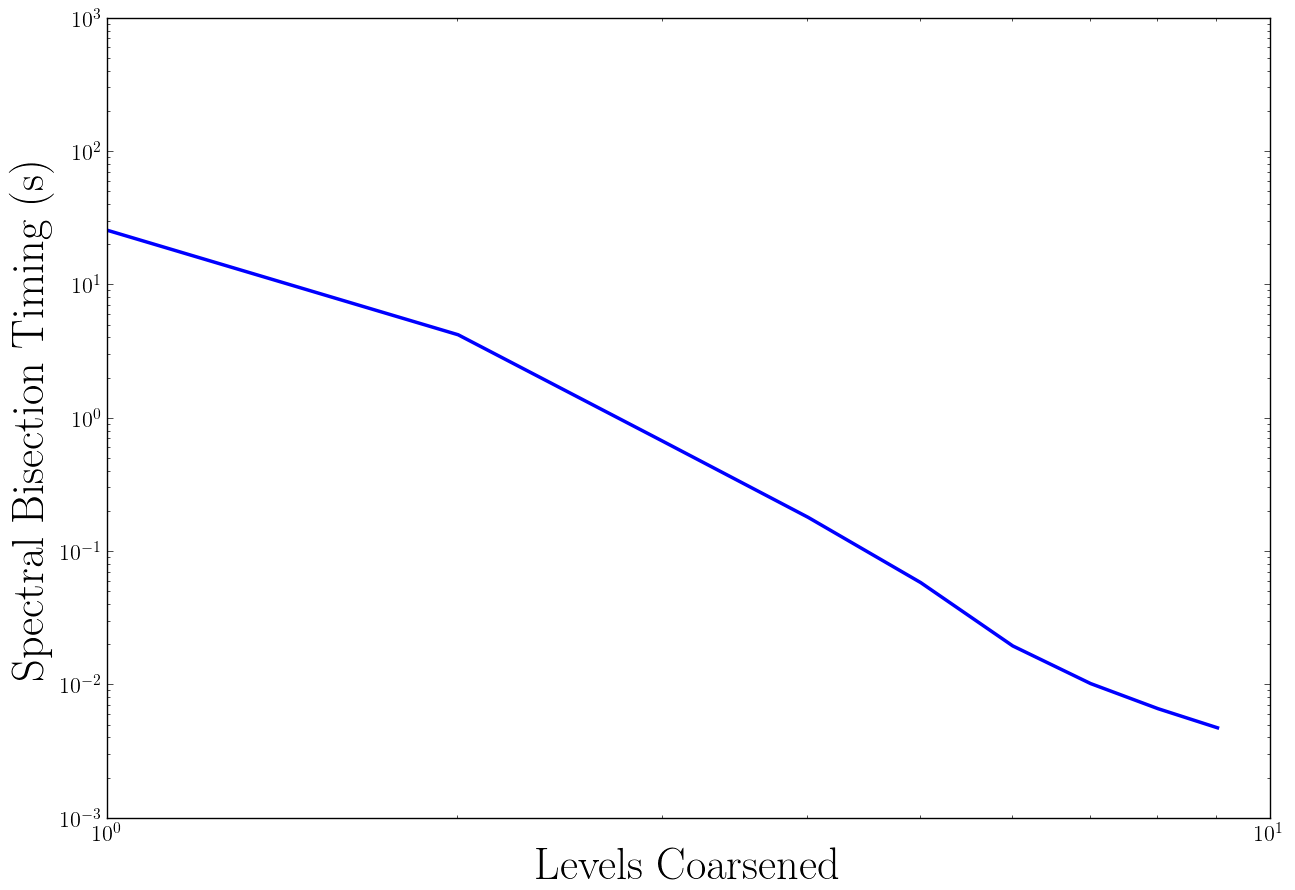
\includegraphics[width=\linewidth]{figs/sbTiming.png}
\end{subfigure}
\begin{subfigure}{.45\textwidth}
        \centering
        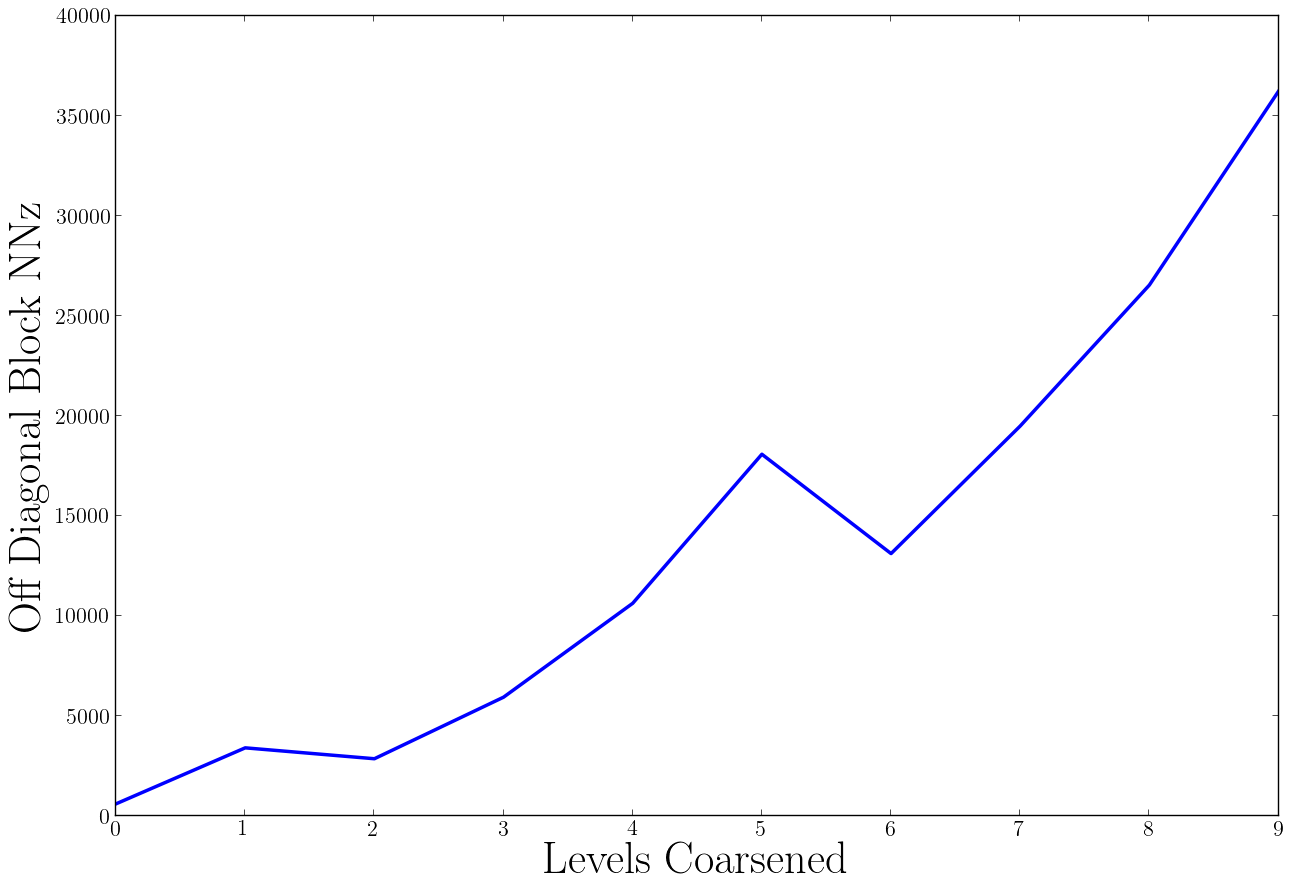
\includegraphics[width=\linewidth]{figs/offDiagNNz.png}
\end{subfigure}
\caption{(Left) Spectral bisection timing (sec) as a function of coarsening
levels before the computation, note logarithmic axes. (Right) Number of nonzeros
in the off diagonal blocks of the final, reordered adjacency matrix after $n$
levels of coarsening, spectral bisection reordering, and uncoarsening to
the granularity of the original graph.}
\label{fig:tradeoff}
\end{figure}

Here we show the sparse Facebook data set to visualize the impact of coarsening
on reordering. The original Facebook data set is shown before reordering in Figure
\ref{fig:FB} (left) and after spectral bisection has been computed without any
coarsening (right). We note here that this result verified that our spectral
bisection algorithm was working properly since this matches what was shown in
class. The original data set has very few nonzeros in the off diagonal block.
However, the spectral bisection reordering reduces this number by roughly an
order of magnitude. 

The plots in Figure \ref{fig:coarseFB}: the left shows the Facebook data after 2
levels of coarsening and reordering, while the right shows this when 9 levels of
coarsening have been applied. Two levels of coarsening still preserves the
Facebook data, and shows a good balance between speed in the spectral bisection
computation with the quality of reordering. Beyond this point however, the
reordering is much worse than the original datset itself. The plot shown after 9
levels of coarsening clearly highlights an extreme case, where the graph is made
up of nearly uniformly distributed clumps.

We show similar a similar visualization for the much larger DBLP data set ($\sim
4.2 \times 10^5$ vertices and $\sim 1$ million edges) in Figures
\ref{fig:DBLPSB} and \ref{fig:DBLP_SB_C4}. Here the number of nonzeros in off
diagonal blocks
is significantly reduced by computing spectral bisection, which is seen by
comparing the left and right
plots of Figure \ref{fig:DBLPSB}. This computation is extremely expensive and
entirely impractical. It is much faster to compute the bisection reordering on a
coarsened graph, but this reduces the quality of the reordering rapidly.
Figure \ref{fig:DBLP_SB_C4} shows the reordering after coarsening the graph only
four times and here the number of nonzeros in the off diagonal blocks is 523194.
This is only slightly reduced from the original data, which had 628800 nonzeros,
thus the reordering is entirely impractical here for reducing communication.

Some of the pitfalls of our coarsening algorithm outlined here can be avoided by
adding a successive refinement scheme, such as those implemented in
\cite{multilevel}. These schemes attack the central problem here: the reordering
associated with a graph coarsened $n$ times is not optimal for the granularity
of the original graph. We did not seek to implement these, however, and found
this implementation informative enough for our purposes. 


\begin{figure}
\centering
\begin{subfigure}{.5\textwidth}
	\centering
	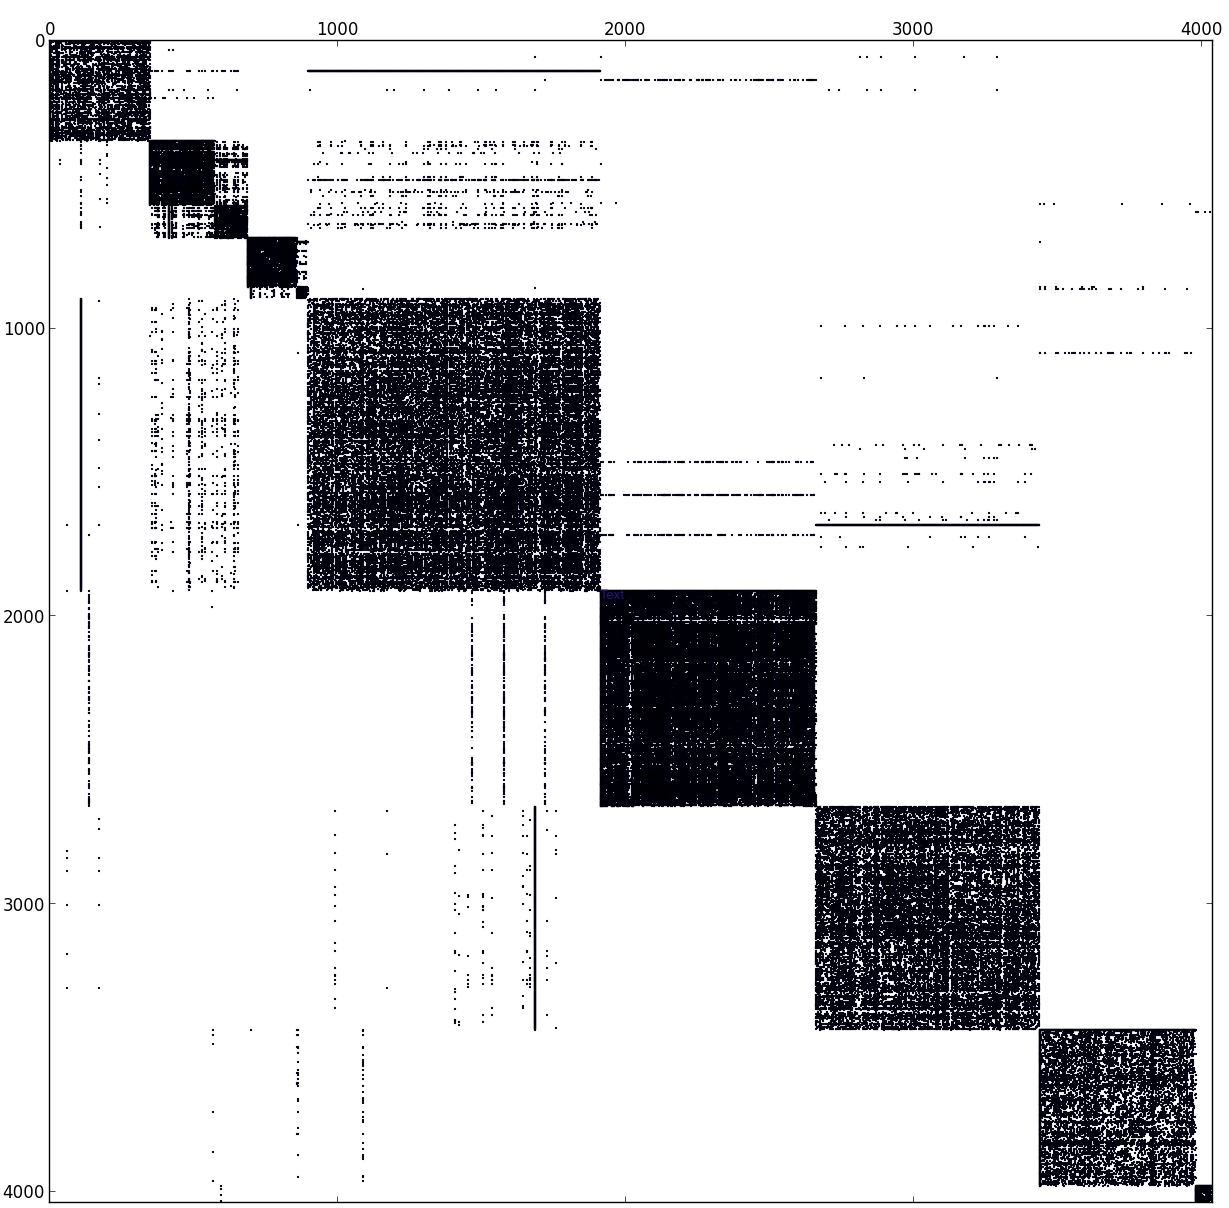
\includegraphics[width=.9\linewidth]{figs/Facebook_Original.png}
	\caption{Original Facebook Data}
	\label{fig:FB}
\end{subfigure}%
\begin{subfigure}{.5\textwidth}
		\centering
		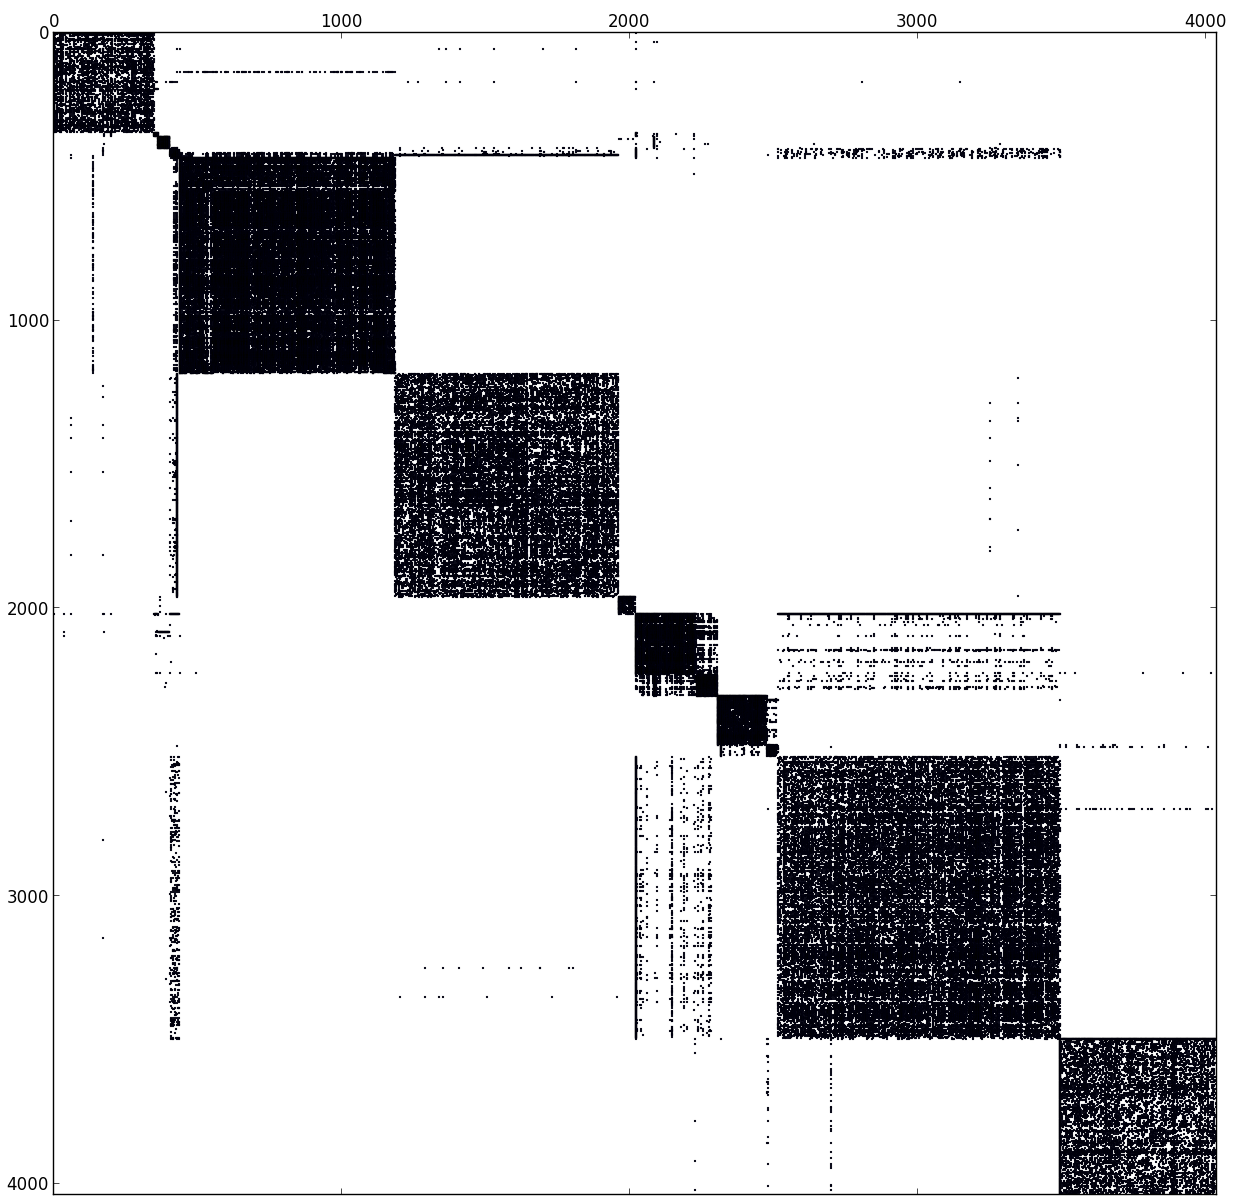
\includegraphics[width=.9\linewidth]{figs/Facebook_SB_C0.png}
		\caption{Facebook Data after Spectral Bisection}
		\label{fig:sub2}
	\end{subfigure}
	\caption{ (a) The original facebook data. Total number of
non-zeros is 88234 and and number of off diagonal non-zeros is 16466. (b)
Facebook data after spectral bisection. The number of off diagonal blocks
reduced to 1266. } 
	\label{fig:FBSB}
\end{figure}


\begin{figure}
\centering
\begin{subfigure}{.5\textwidth}
	\centering
	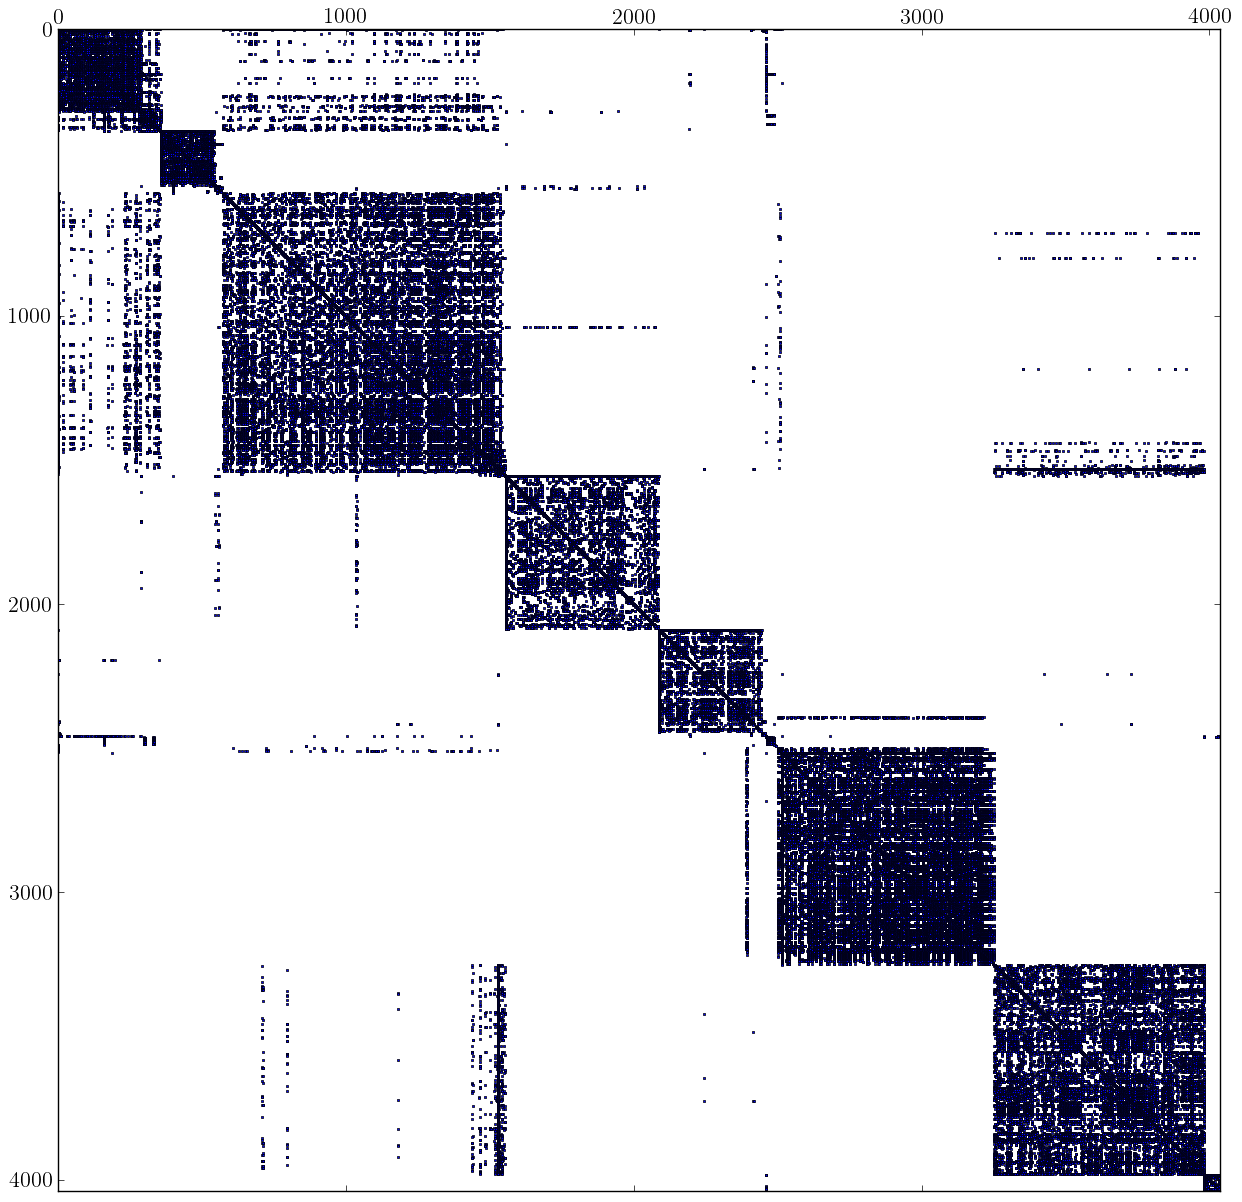
\includegraphics[width=.9\linewidth]{figs/Facebook_c2.png}
	\caption{Facebook Data after 2 levels of coarsening}
	\label{fig:FB2}
\end{subfigure}%
\begin{subfigure}{.5\textwidth}
		\centering
		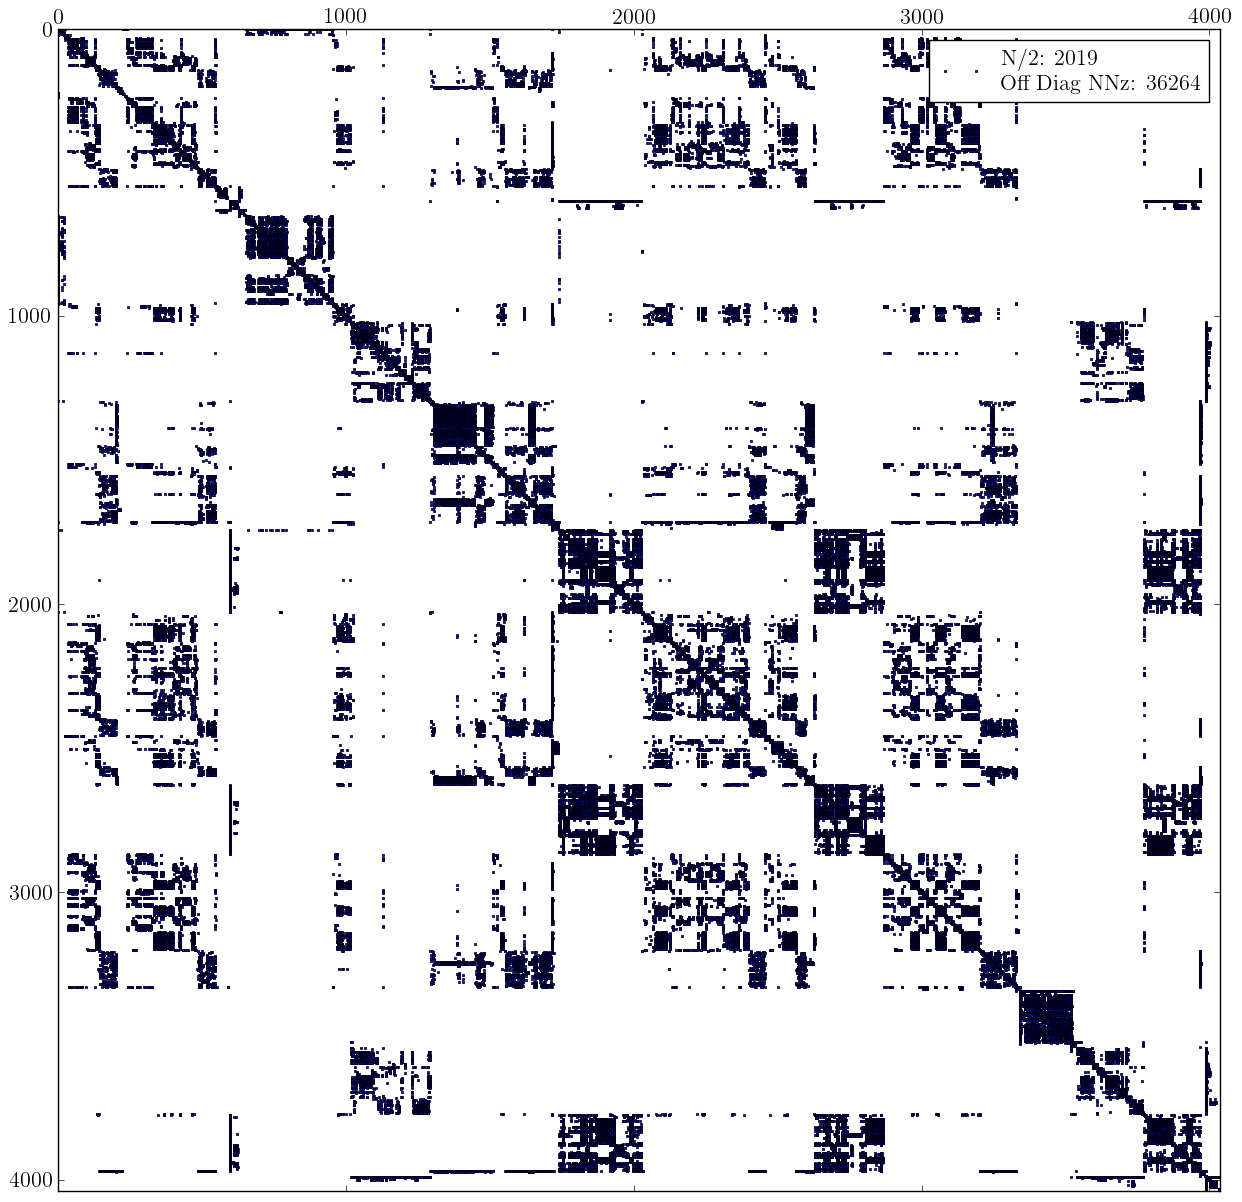
\includegraphics[width=.9\linewidth]{figs/Facebook_c9.png}
		\caption{Facebook Data after 9 levels of coarsening}
		\label{fig:FB9}
	\end{subfigure}
	\caption{ Same as \ref{fig:FBSB} but where spectral bisection was
computed after 2 (left) and 9 (right) levels of coarsening. The total off
diagonal nonzeros is 5774 (left) and 72528 (right). } 
	\label{fig:coarseFB}
\end{figure}



%%%%%%%%%%%% strong scaling
\subsection{Coarsening Strong Scaling on KNL: DBLP data}

Here we tested the scaling of our coarsening algorithm implementation on a single
Knights Landing node with the DBLP data set ($\sim 420000$ vertices and $\sim 1$
million edges). Clearly the most expensive stage of the coarsening algorithm is
the first one, since each successive step afterward has fewer nodes and edges.
Thus we simply tested the timing for completing this first stage across varying
levels of threads. These timing results are shown in Figure
\ref{fig:color_time}. The coloring took the most time to complete, dwarfing the
computations associated with maximal matching. The time drops exponentially to
roughly 32 threads on the node, and increases again at 68 and 272 threads. We
note that since the KNL nodes have 68 cores, up to this thread count there is
one thread per physical core. There are up to four logical threads per core,
allowing for 272 threads. However there is clearly substantial time wasted in
overhead since this is clearly more expensive than both with 32 and 68 threads.

With only one million elements to work with in compressed storage, the data that
we are working with only requires on the order of megabytes of storage. It makes
sense that the algorithm does not scale to a large number of threads since they
would each be caught up in communication overhead rather than computation. This
is what we see after 32 threads. The slow down beyond this point is probably due
to latency from processors communicating across more than half of the socket.

We note also that we tested the coarsening algorithm on both flat and cache
memory models of the KNL node. The node has about 100GB of DDR4 RAM, at 90 GB/s
bandwidth, and 16 GB of MCDRAM at up to 475 GB/s. The cache mode is the default
memory model for KNL which hides the fast MCDRAM to the user such that it acts
as a high level cache. In flat mode, the user can control data elements which
live in MCDRAM. Since our application took advantage of sparse storage schemes,
the memory footprint was well under 1GB, allowing us to flexibly try both modes.
We found no difference between the flat and cache mode, which is likely because
the size of our application was so small that it could fit in MCDRAM regardless
of the memory configuration.

Despite decent scaling to 32 cores (threads), the coarsening and reordering
algorithms are far
too expensive to even be considered for any practical implementation because
solving the linear system in Eqn. (\ref{eq:pagerank_linear}) is extremely fast
with the write data format. We discuss these results in the next subsection.

\begin{figure}
\centering
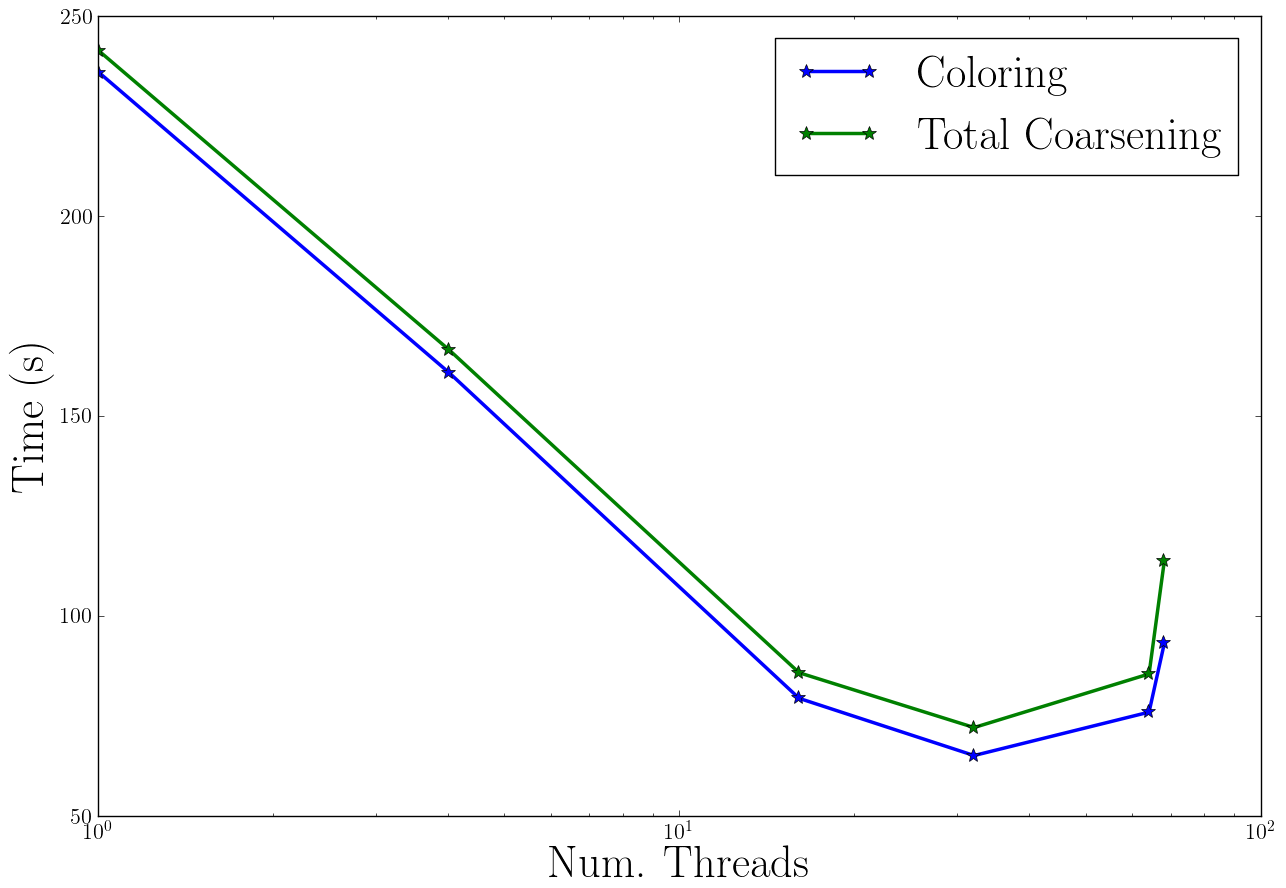
\includegraphics[width=.5\linewidth]{figs/color_timing.png}
\caption{Strong scaling of the coarsening algorithm (Coloring and Maximal
Matching) in shared memory on a single Knights Landing node. Note the
logarithmic x-axis.}
\label{fig:color_time}
\end{figure}


\subsection{Solving the PageRank problem with the DBLP Dataset}

To test our methodology on a larger data set, we make use of the DBLP
collaboration network data set \cite{snapnets,dblp}. This is the same data used
in \cite{xie} to test their low-rank approximation algorithm; they compute 1000
samples offline (i.e., solve the page rank problem 1000 times) in order to find a
low dimensional subspace for the least squares problems described in section 1.
The times given in \cite{xie} for
computing these samples and finding a basis for the low dimensional subspace 
is given in table \ref{tab:time}.

\begin{table}[h!]
	\centering 
\captionof{table}{Time estimates given in \cite{xie}}
   \begin{tabular}[h]{|l|c|c|c|}
	   \hline 
	   \textbf{Procedure} & \textbf{DBLP} & \textbf{Weibo-G} &
	   \textbf{Weibo-L} \\
	   \hline
	   Prepare Samples & 6 hours & 17 hours & 3-7 min \\ 
	   Get Basis $U^*$ & 0.8 hours & 0.4 hours & 1-2 min \\
	   \hline
   \end{tabular}
\label{tab:time}
\end{table}

\begin{table}[h!]
	\centering
	\captionof{table}{Iterative Solve Time on KNL in sec}
	\begin{tabular}[h]{|c||c|c|c|c|}
		\hline
		Cores/Threads& 1 & 16 & 64 & 272 \\
		\hline
		Original Data & 7.36 & 7.63 & 7.64 & 7.71\\
		Spectral Bisection & 7.24 & 7.74 & 7.76 & 7.57 \\
		\hline
		Parallel Matvec & \multicolumn{4}{|c|}{$\approx$ 0.09}\\
		\hline
	\end{tabular}
\label{tab:KNLTIME}
\end{table}

\begin{table}[h!]
	\centering
	\captionof{table}{Iterative Solve Time on ICES in sec}
	\begin{tabular}[h]{|l||c|c|c|c|}
		\hline
		Cores & 1 & 2& 3 & 4 \\
		\hline
		Original Data & 1.55 & 1.56 & 1.56 & 1.57\\
		Spectral Bisection & 1.45 & 1.55 & 7.53 & 1.54 \\
		\hline
		Parallel Matvec & \multicolumn{4}{|c|}{$\approx$ 0.02}\\
		\hline
	\end{tabular}
\label{tab:ICESTIME}
\end{table}

Even though computing the spectral bisection of the DBLP data with or without
coarsening is infeasible, these results provide an opportunity to test how
effective spectral bisection is at speeding up the matvec in the iterative
solver. Using algorithm
\ref{CSC} we solve the page rank problem using the original DBLP data, and the
reordered DBLP data shown in figures \ref{fig:DBLP} and \ref{fig:DBLP_SB_C0},
respectively. We test the solvers on Intel's KNL nodes on Stampede 2, and on one
of our desktops (4 cores at 3.3GHz). The timing results for the page rank
problem on the different
machines and on multiple cores are shown in table \ref{tab:KNLTIME} and
\ref{tab:ICESTIME}.

In both cases, solving the linear system with the original data
or wth the spectral bisection reordered data produces the same result. The true
speed up comes from using CSC format. As mentioned early, this significantly
reduces the storage cost as well as the number of computations needed. The
spectral bisection results would probably make a difference with distributed
memory, or perhaps if we performed recursive spectral bisection; however, the
speed up appears to be minimal on shared memory. We note here that our
implementation produced the same times on both flat and cache mode on the KNL
processors. We suspect this is because the vectors being applied are so small
that they can fit in the MCDRAM no matter how the memory is configured.

Our sparse matvec calculations significantly beat the times given in \cite{xie}.
We could solve 1000 page rank
problems in about 25 minutes for the DBLP data as opposed to the 6 hours taken
in \cite{xie}. 


\begin{figure}
\centering
\begin{subfigure}{.5\textwidth}
	\centering
	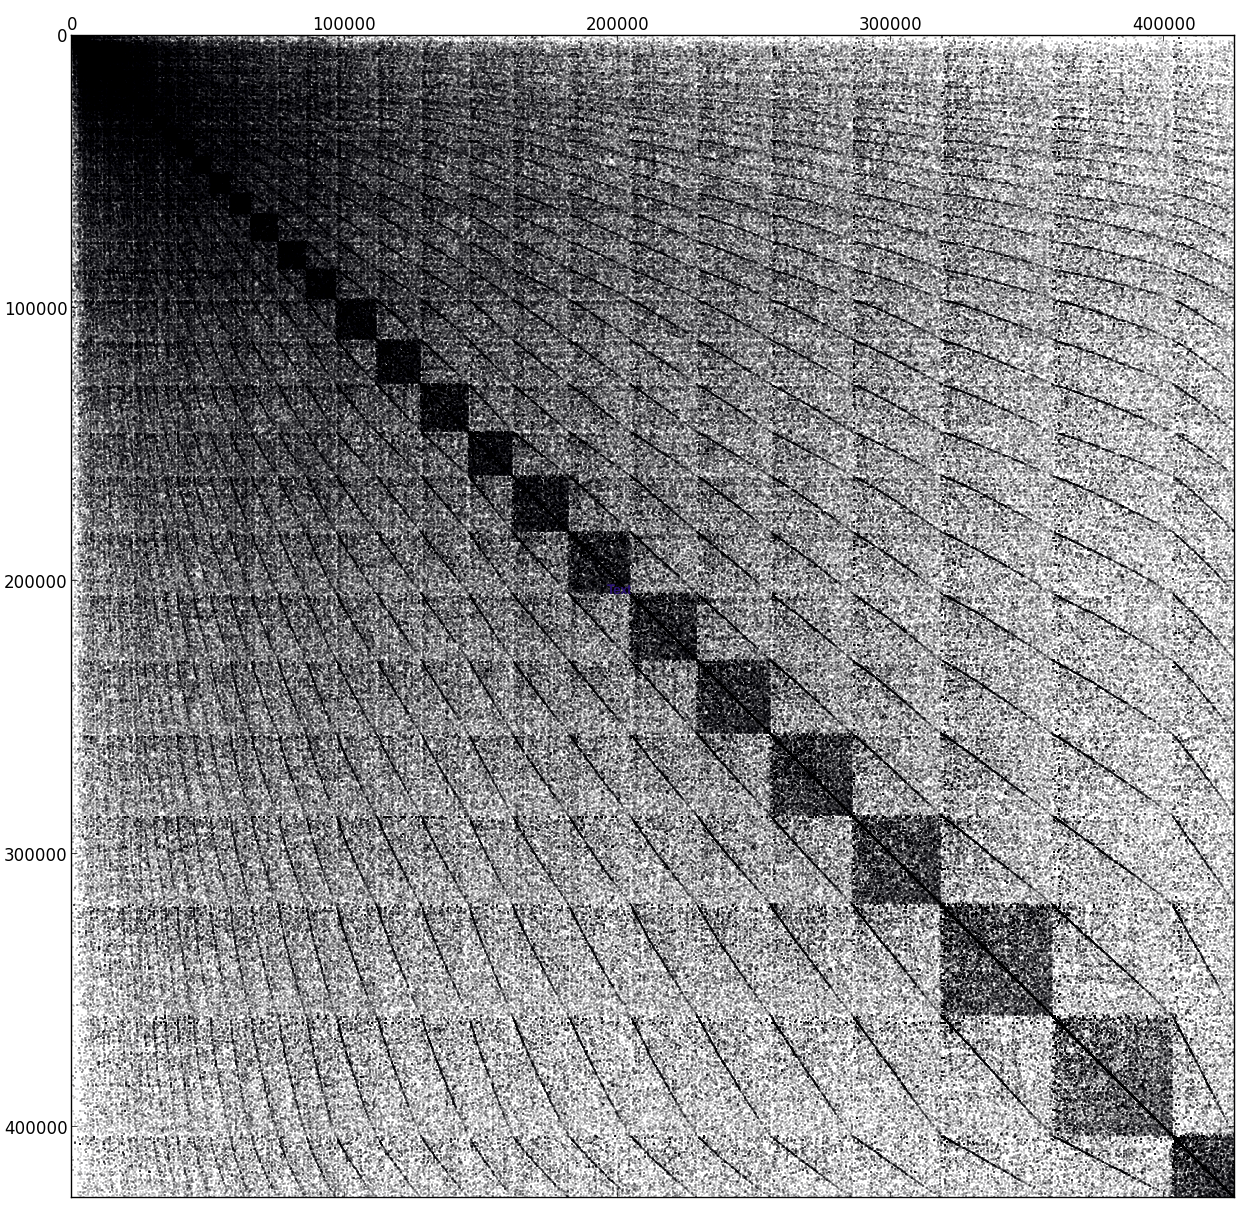
\includegraphics[width=.9\linewidth]{figs/DBLP_Original.png}
	\caption{DBLP Original Data}
	\label{fig:DBLP}
\end{subfigure}%
\begin{subfigure}{.5\textwidth}
		\centering
		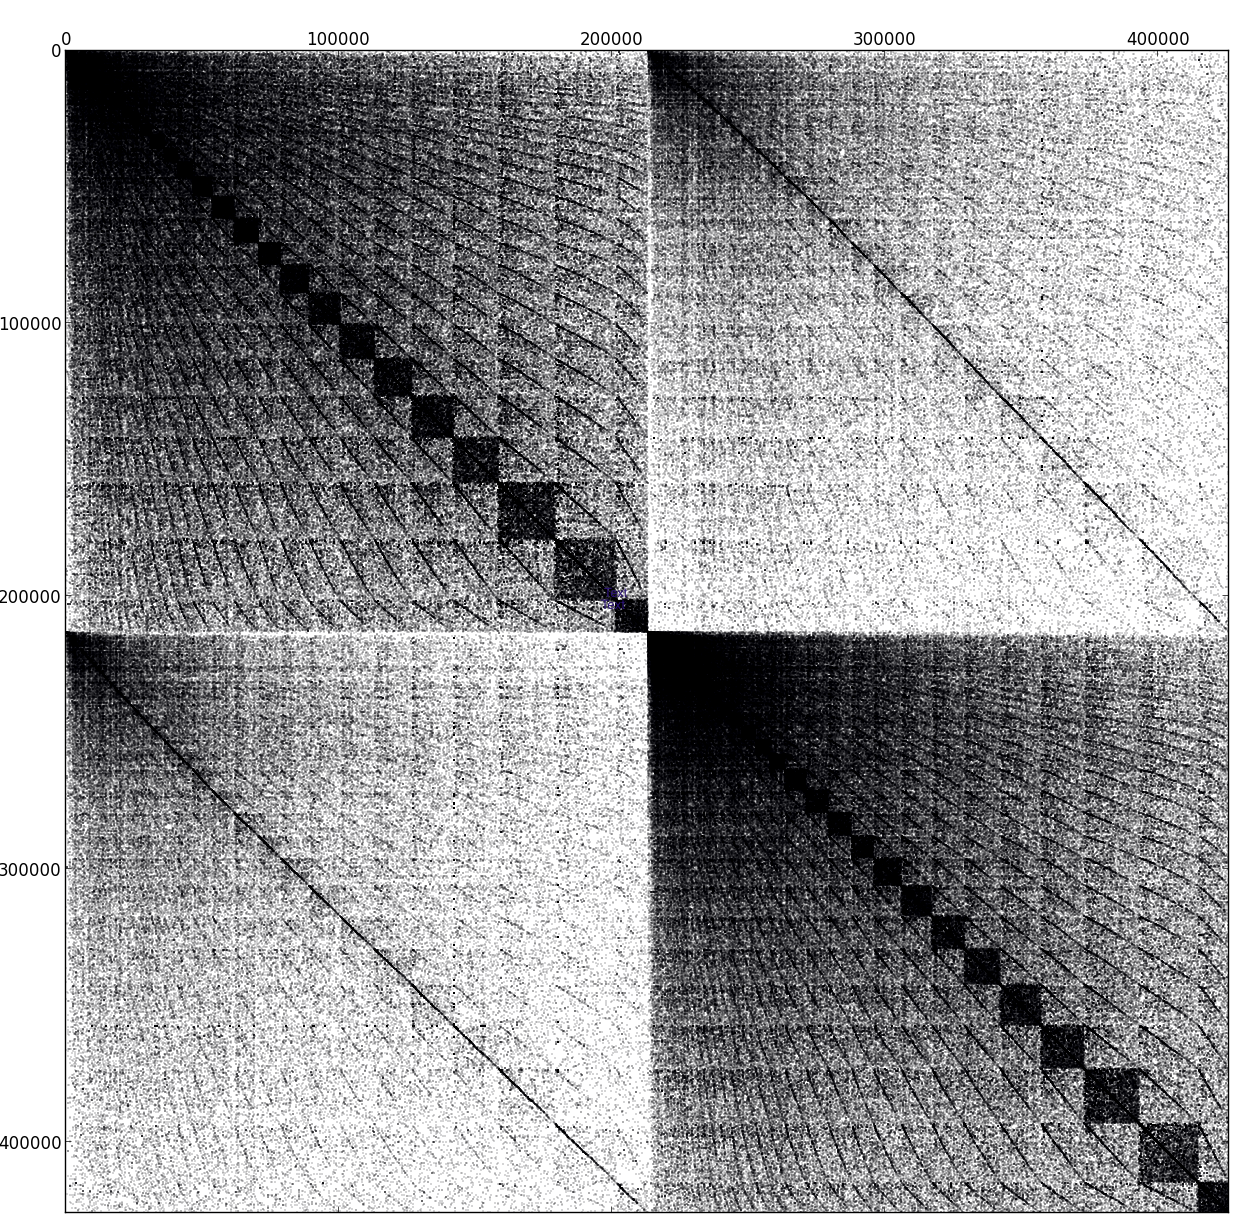
\includegraphics[width=.9\linewidth]{figs/DBLP_SBC0.png}
		\caption{DBLP after Spectral Bisection}
		\label{fig:DBLP_SB_C0}
	\end{subfigure}
	\caption{ (a) The original DBLP data. Total number of
non-zeros is 1049866 and and number of off diagonal non-zeros is 628800. (b)
DBLP data after spectral bisection. The number of off diagonal blocks
reduced to 350038. } 
	\label{fig:DBLPSB}
\end{figure}

\begin{figure}
	\centering
	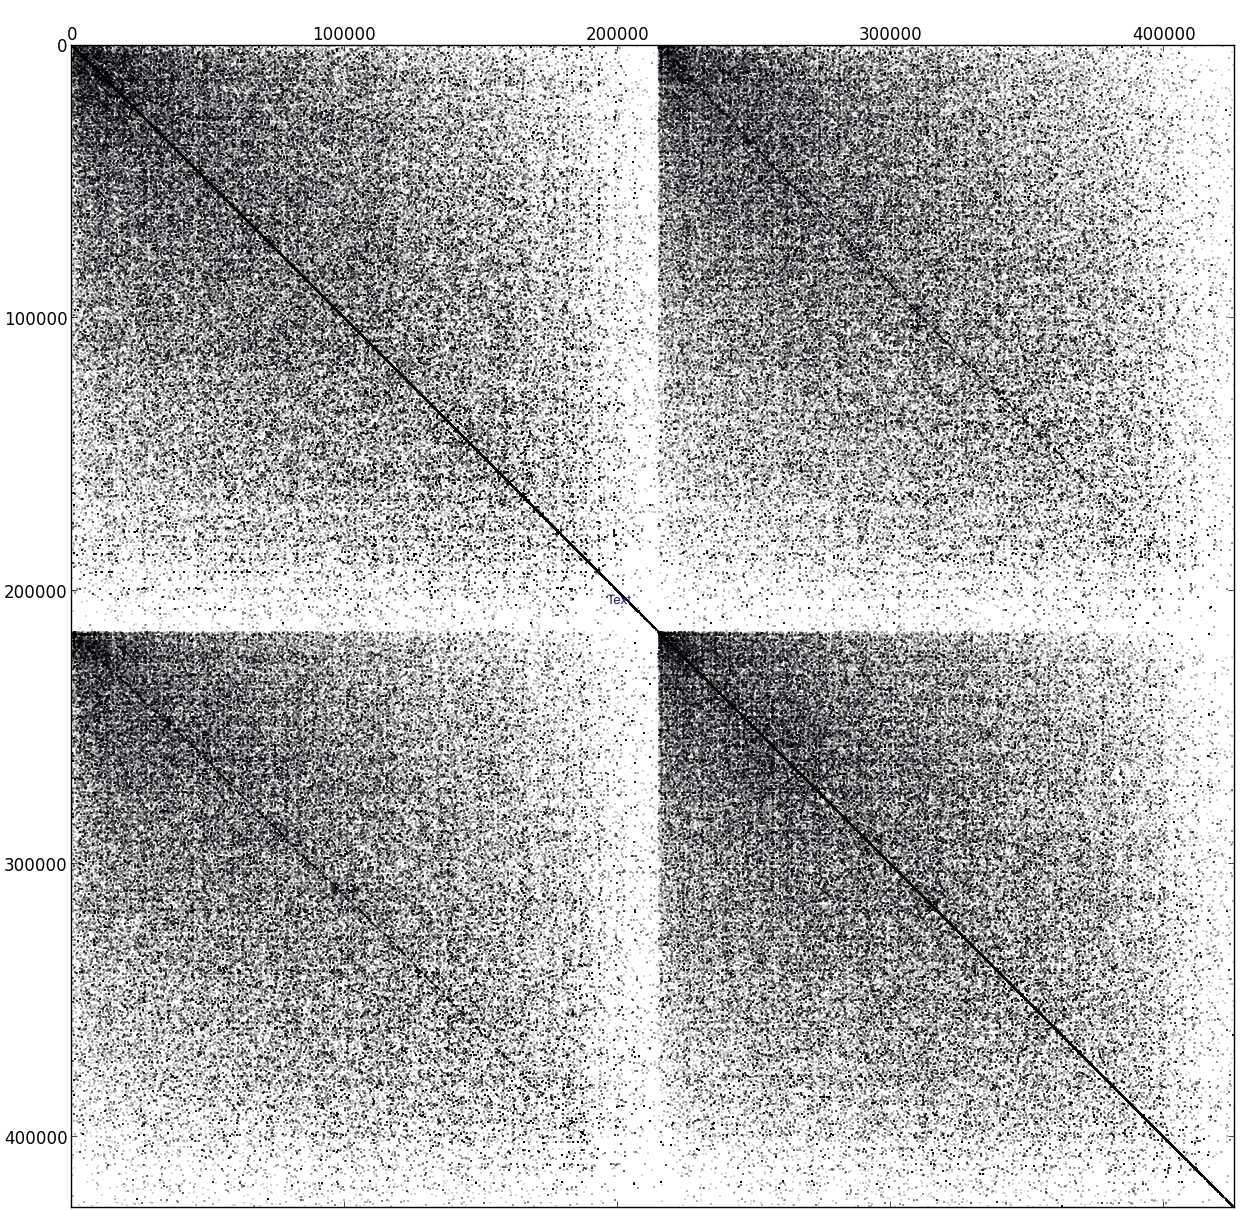
\includegraphics[width=0.5\linewidth]{figs/DBLP_SBC4.png}
	\caption{DBLP data after four coarsens and then spectral bisection. The
	number of off diagonals reduced slightly to 523194.}
	\label{fig:DBLP_SB_C4}
\end{figure}






%%%%%%%%%%%%%%%%%%%%%%%%%%%%%%%%%%%%%%%%%%%%%%%%%%%%%%
% CITATIONS
%%%%%%%%%%%%%%%%%%%%%%%%%%%%%%%%%%%%%%%%%%%%%%%%%%%%%%%%%%%
\newpage

%\addcontentsline{toc}{subsubsection}{\protect\numberline{\thesubsubsection}
%  line added to TOC: subsubsection one}

\addcontentsline{toc}{section}{References} 

\bibliographystyle{ieeetr} 
\bibliography{spicy}



\end{document}

